\documentclass[a4paper,11pt]{article}

% Packages, page layout, and shared figure/table style for the report.

\usepackage[T1]{fontenc}
\usepackage[
    a4paper,
    top=0.85in,
    bottom=0.85in,
    left=0.65in,
    right=0.65in,
    headheight=15pt,
    headsep=10pt,
    footskip=25pt
]{geometry}
\usepackage{amsmath}
\usepackage{booktabs}
\usepackage{caption}
\usepackage{enumitem}
\usepackage{fancyhdr}
\usepackage{float}
\usepackage{graphicx}
\usepackage{listings}
\usepackage{multicol}
\usepackage{titlesec}
\usepackage{verbatim}
\usepackage{xcolor}
\usepackage[bottom]{footmisc}
\usepackage[hidelinks]{hyperref}

\graphicspath{{figures/}}
\raggedbottom

% Plot and table on one row, captions on the next.
% #1 plot  #2 figure caption  #3 table  #4 table caption
% [c] centers the table against the plot, not the plot+caption block.
\newcommand{\plotandtable}[4]{%
    \noindent
    \begin{minipage}[c]{0.55\textwidth}
        \centering
        #1
    \end{minipage}%
    \hfill
    \begin{minipage}[c]{0.42\textwidth}
        \centering
        #3
    \end{minipage}\\[2pt]
    \noindent
    \begin{minipage}[t]{0.55\textwidth}
        \centering
        \captionsetup{skip=0pt, belowskip=0pt}
        #2
    \end{minipage}%
    \hfill
    \begin{minipage}[t]{0.42\textwidth}
        \centering
        \captionsetup{skip=0pt, belowskip=0pt}
        #4
    \end{minipage}%
}

\setlength{\parindent}{0pt}
\setlength{\parskip}{7pt}

\pagestyle{fancy}
\fancyhf{}
\lhead{ESE 507}
\chead{Project Part 1}
\rhead{Jin Y. Chen}
\cfoot{\thepage}
\renewcommand{\headrulewidth}{0.4pt}
\renewcommand{\footrulewidth}{0pt}
\fancypagestyle{plain}{\fancyhf{}\renewcommand{\headrulewidth}{0pt}\cfoot{\thepage}}

\titleformat{\section}{\large\bfseries}{\thesection.}{0.5em}{}
\titleformat{\subsection}{\normalsize\bfseries}{\thesubsection.}{0.5em}{}
\titlespacing*{\section}{0pt}{12pt}{6pt}
\titlespacing*{\subsection}{0pt}{10pt}{4pt}

\captionsetup{
    font=small,
    labelfont=bf,
    skip=4pt,
    belowskip=2pt
}
\setlength{\intextsep}{8pt plus 2pt minus 2pt}
\setlength{\textfloatsep}{8pt plus 2pt minus 2pt}

% Keep deferred tables at the top of the page instead of vertically
% centering them on a float-only page (large empty header margin).
\makeatletter
\setlength{\@fptop}{0pt}
\setlength{\@fpsep}{8pt plus 2pt minus 2pt}
\setlength{\@fpbot}{0pt plus 1fil}
\makeatother

\definecolor{codebg}{RGB}{245,247,250}
\definecolor{codeblue}{RGB}{0,92,153}
\definecolor{codegreen}{RGB}{40,120,75}
\definecolor{codepurple}{RGB}{125,60,150}
\definecolor{codegray}{RGB}{90,90,90}

\lstdefinestyle{Verilog}{
    language=Verilog,
    backgroundcolor=\color{codebg},
    basicstyle=\ttfamily\small,
    keywordstyle=\color{codeblue}\bfseries,
    commentstyle=\color{codegreen}\itshape,
    stringstyle=\color{codepurple},
    numbers=left,
    numberstyle=\tiny\color{codegray},
    numbersep=8pt,
    frame=single,
    framesep=5pt,
    rulecolor=\color{gray!40},
    breaklines=true,
    showstringspaces=false,
    tabsize=4,
    xleftmargin=10pt,
    framexleftmargin=10pt
}

% ==================================================
% Document
% ==================================================

\begin{document}

% ==================================================
% Title Page
% ==================================================

\hypersetup{pageanchor=false}
\begin{titlepage}

\centering

\vspace*{1.5in}

{\Large ESE 507\par}

\vspace{0.5in}

{\Huge\bfseries Project: Part 1\par}

\vspace{1in}

{\large
Jin Yuan Chen\\[0.25em]
115702978
\par}

\vfill

{\large \today\par}

\end{titlepage}
\hypersetup{pageanchor=true}

% \section{Introduction}

% \subsection{Overview}

% \subsection{Specification}

% \subsection{Architecture}


\clearpage
\pagenumbering{roman}
\tableofcontents
\clearpage
\pagenumbering{arabic}

\section{Multiply Accumulate (MAC) Design}

Two versions of the MAC were implemented to compare the unpipelined and pipelined designs. Both the unpipelined \texttt{mac} and pipelined \texttt{mac\_pipe} designs use an accumulator register that updates its output on the rising edge of the clock. The primary difference between the two designs is the combinational multiply-add operation. In the unpipelined \texttt{mac}, the multiplication and addition are performed within a single combinational stage before the result is stored in the accumulator. In the pipelined \texttt{mac\_pipe}, the multiply-add operation is divided into two stages. The multiplier output and associated control signals are stored in an additional intermediate register before the addition is performed and the result is stored in the accumulator on the following clock cycle. Consequently, the pipelined design introduces an additional cycle of latency, requiring two clock cycles for an input to propagate to the accumulator output, compared with one cycle for the unpipelined design. However, the benefits of pipelining become apparent when considering the overall throughput and frequency of the system. 

\subsection{Design Parameter}
Both the \texttt{mac} and \texttt{mac\_pipe} designs were synthesized with \texttt{WIDTH = 16} and \texttt{ACCW = 48} across a range of clock frequencies. The analysis spans frequencies from a relatively low frequency of 10~MHz to a maximum of 1~GHz. At each frequency, the area, power, critical path location, and timing constraint of each design are evaluated.

\clearpage
\section{Combinational Synthesis Results}

The unpipelined \texttt{mac} design was synthesized to determine the maximum achievable clock frequency with \texttt{WIDTH = 16} and \texttt{ACCW = 48}. The synthesis workflow was automated with scripts that write the configured design parameters and the synthesis script, before running synthesis on the remote CAD server. The generated synthesis report is filtered for key attributes, including area, power, and timing. For convenient data analysis, these attributes are stored in comma-separated value (CSV) files for every synthesis run. The tabular structure of the CSV files is well suited for Python plotting libraries, which were used to generate the graphs below. For more details on the automation workflow, refer to \texttt{scr/}. Only data points that \textbf{meet the timing constraint} are plotted in the graphs below.

% For each frequency you try, record the area, power, the critical path location, and whether the timing 
% constraint was met or violated.

% make a table that shows this data for each attempted 
% frequency.  

%Make  sure  you  include  units  on  all  values  you  report 

\subsection{Area}

The design area is estimated from the synthesis report as the total cell area, which does not account for net interconnect area. Therefore, the actual physical area of the design with interconnects may be larger than the reported area. Further analysis of design area uses the conservative estimation as the sum of combinational area, buffer/inverter area, noncombinational area and macro/black box area in the synthesis report.


As shown in Figure~\ref{fig:mac-area}, the total design area remains relatively constant as the frequency increases. However, an overall upward trend is seen, particularly at frequencies above 200~MHz. This increase can be attributed to the additional area required to meet the more difficult timing constraints associated with higher frequency. The approximately linear increase in area beyond 200~MHz indicates the achievable trade-off for frequency at the expensive of area. In contrast, the relatively constant area at lower frequencies suggests that the synthesis tool implemented the design to a near-minimal cell configuration regardless of less restrictive timing constraints. 

\begin{figure}[!htbp]
    \plotandtable{%
        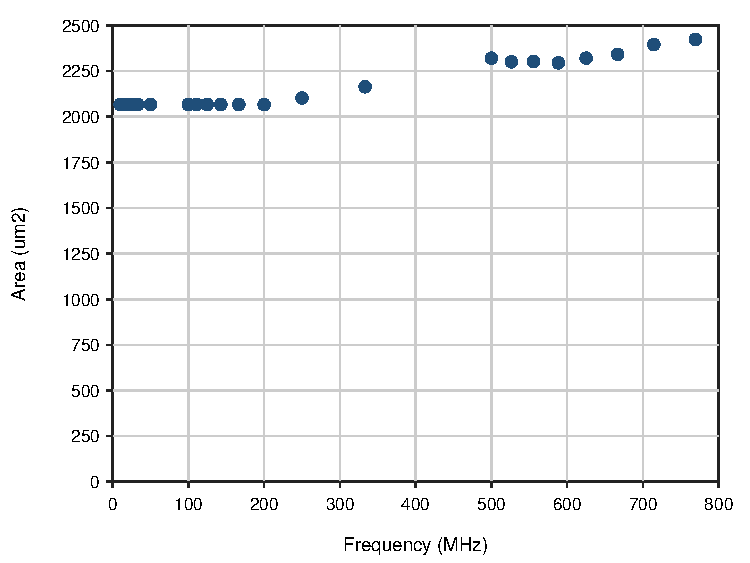
\includegraphics[width=\linewidth]{mac_freq_MHz_area_um2_MET.pdf}
    }{%
        \caption{Area, frequency for unpipelined \texttt{mac} (MET).}
        \label{fig:mac-area}
    }{%
        \scriptsize
        \begin{tabular}{rr}
            \toprule
            \textbf{Freq.\ (MHz)} & \textbf{Area ($\mu m^2$)} \\
            \midrule
            10     & 2067.09 \\
            20     & 2067.09 \\
            25     & 2067.09 \\
            50     & 2067.09 \\
            100    & 2067.09 \\
            166.67 & 2067.09 \\
            200    & 2066.29 \\
            333.33 & 2164.18 \\
            $\vdots$ & $\vdots$ \\
            500    & 2320.85 \\
            526.32 & 2300.90 \\
            555.56 & 2302.76 \\
            769.23 & 2424.06 \\
            \bottomrule
        \end{tabular}
    }{%
        \captionof{table}{Selected MET area points for \texttt{mac}.}
        \label{tab:mac-area}
    }
\end{figure}
 

An interesting pattern is the occasional small downward trend in area at higher frequencies. This suggests that, at certain frequency, the synthesis tool may identify a simplified version that meets timing constraint with less cell area. For example, the design synthesized at 555.56~MHz has a slightly lower total area than the design synthesized at 500~MHz, despite the overall increasing trend of frequency and area. This behavior indicates that the relationship between frequency and synthesized area is not strictly monotonic and can depend on the specific optimizations selected by the synthesis tool.

\subsection{Power}

The Total Power shown in Figure~\ref{fig:mac-power} is defined as the sum of Total Dynamic Power and Cell Leakage Power in the synthesis report. The Total Dynamic Power is also reported as the sum of Cell Internal Power and Net Switching Power, both contributing an near equal portion of the sum. 

\begin{figure}[!htbp]
    \plotandtable{%
        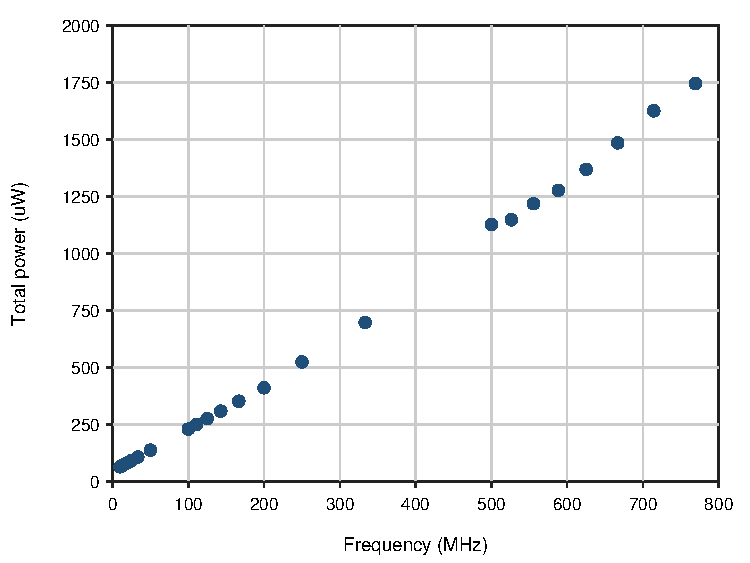
\includegraphics[width=\linewidth]{mac_freq_MHz_total_uw_MET.pdf}
    }{%
        \caption{Total power, frequency for unpipelined \texttt{mac} (MET).}
        \label{fig:mac-power}
    }{%
        \scriptsize
        \begin{tabular}{rr}
            \toprule
            \textbf{Freq.\ (MHz)} & \textbf{$\sum$ Power ($\mu W$)} \\
            \midrule
            10     & 65.49 \\
            20     & 83.85 \\
            25     & 93.03 \\
            50     & 138.92 \\
            100    & 230.72 \\
            166.67 & 353.12 \\
            200    & 411.86 \\
            333.33 & 698.23 \\
            $\vdots$ & $\vdots$ \\
            500    & 1127.93 \\
            526.32 & 1148.45 \\
            555.56 & 1218.61 \\
            769.23 & 1745.19 \\
            \bottomrule
        \end{tabular}
    }{%
        \captionof{table}{Selected MET power points for \texttt{mac}.}
        \label{tab:mac-power}
    }
\end{figure}

The Cell Leakage Power is almost negligible compared with the dynamic power. This may be attributed to the relatively small area of the design, with the accumulator register being the primary memory elements contributing to leakage power. In the case that the frequency is considerably slow, the dynamic power can become sufficiently small that leakage power becomes a significant contributor to total power. Otherwise, given a fixed accumulator width and integer-bit width, the leakage power remains approximately constant at frequency below 166.67 MHz, as shown in the table of Figure 1. This suggests that leakage power is primarily dependent on the area of the design. The slight increase in leakage power at higher frequencies can therefore be attributed to the corresponding increase in design area.

Consequently, the trend seen in Figure~\ref{fig:mac-power} for total power is largely influenced by the Dynamic Power and its dependence on frequency. Increasing the frequency results in a near linear increase in Dynamic Power, with an approximate power increase of 1.836 $\mu\text{W}/\text{MHz}$. In other words, a higher-frequency design performs more switching operation per unit time than a lower-frequency design, resulting in higher power consumption over the same period of time. 


\subsection{Critical Paths}

The synthesis report provides the start and end points of the critical paths, along with the paths themselves and their data arrival times. If the data arrival time is less than or equal to the data required time, the design constraint is considered MET, as indicated by Slack (MET) in the report.

A design with Slack (VIOLATED) indicates a timing constraint violation and will typically display a negative slack value, calculated as the difference between the data arrival time and the data required time. A negative value indicates that the timing constraint has not been met. A design reported as Slack (VIOLATED: increase significant digits) is also considered a violation, even if the displayed slack value is zero. This occurs because the actual slack value is slightly negative but is rounded to zero due to the limited number of significant digits displayed in the report.

\begin{table}[H]
    \centering
    \scriptsize
    \begin{tabular}{rrrrlll}
        \toprule
        \textbf{Freq.\ (MHz)} &
        \textbf{Area ($\mu m^2$)} &
        \textbf{Power ($\mu W$)} &
        \textbf{Slack (ns)} &
        \textbf{Path Start} &
        \textbf{Path End} &
        \textbf{Timing} \\
        \midrule
        10      & 2067.09 & 65.49   & 95.68  & \texttt{input0[1]}  & \texttt{acc\_reg[47]} & MET \\
        11.11   & 2067.09 & 67.53   & 85.68  & \texttt{input0[1]}  & \texttt{acc\_reg[47]} & MET \\
        12.5    & 2067.09 & 70.08   & 75.68  & \texttt{input0[1]}  & \texttt{acc\_reg[47]} & MET \\
        14.29   & 2067.09 & 73.35   & 65.68  & \texttt{input0[1]}  & \texttt{acc\_reg[47]} & MET \\
        16.67   & 2067.09 & 77.73   & 55.68  & \texttt{input0[1]}  & \texttt{acc\_reg[47]} & MET \\
        20      & 2067.09 & 83.85   & 45.68  & \texttt{input0[1]}  & \texttt{acc\_reg[47]} & MET \\
        25      & 2067.09 & 93.03   & 35.68  & \texttt{input0[1]}  & \texttt{acc\_reg[47]} & MET \\
        33.33   & 2067.09 & 108.32  & 25.68  & \texttt{input0[1]}  & \texttt{acc\_reg[47]} & MET \\
        50      & 2067.09 & 138.92  & 15.68  & \texttt{input0[1]}  & \texttt{acc\_reg[47]} & MET \\
        100     & 2067.09 & 230.72  & 5.68   & \texttt{input0[1]}  & \texttt{acc\_reg[47]} & MET \\
        111.11  & 2067.09 & 251.12  & 4.68   & \texttt{input0[1]}  & \texttt{acc\_reg[47]} & MET \\
        125     & 2067.09 & 276.62  & 3.68   & \texttt{input0[1]}  & \texttt{acc\_reg[47]} & MET \\
        142.86  & 2067.09 & 309.40  & 2.68   & \texttt{input0[1]}  & \texttt{acc\_reg[47]} & MET \\
        166.67  & 2067.09 & 353.12  & 1.68   & \texttt{input0[1]}  & \texttt{acc\_reg[47]} & MET \\
        200     & 2066.29 & 411.86  & 0.68   & \texttt{input0[1]}  & \texttt{acc\_reg[47]} & MET \\
        250     & 2102.20 & 525.46  & 0.01   & \texttt{input0[0]}  & \texttt{acc\_reg[47]} & MET \\
        333.33  & 2164.18 & 698.23  & 0.00   & \texttt{input0[7]}  & \texttt{acc\_reg[47]} & MET \\
        500     & 2320.85 & 1127.93 & 0.00   & \texttt{input0[3]}  & \texttt{acc\_reg[47]} & MET \\
        526.32  & 2300.90 & 1148.45 & 0.03   & \texttt{input0[5]}  & \texttt{acc\_reg[47]} & MET \\
        555.56  & 2302.76 & 1218.61 & 0.00   & \texttt{input0[7]}  & \texttt{acc\_reg[47]} & MET \\
        588.24  & 2295.58 & 1277.55 & 0.01   & \texttt{input0[11]} & \texttt{acc\_reg[47]} & MET \\
        625     & 2321.12 & 1369.41 & 0.00   & \texttt{input0[5]}  & \texttt{acc\_reg[47]} & MET \\
        666.67  & 2341.60 & 1485.30 & 0.00   & \texttt{input0[5]}  & \texttt{acc\_reg[44]} & MET \\
        714.29  & 2395.60 & 1626.06 & 0.00   & \texttt{input0[0]}  & \texttt{acc\_reg[35]} & MET \\
        769.23  & 2424.06 & 1745.19 & 0.00   & \texttt{input0[7]}  & \texttt{acc\_reg[31]} & MET \\
        833.33  & 2471.14 & 2003.27 & $-0.07$ & \texttt{input0[5]}  & \texttt{acc\_reg[33]} & VIOLATED \\
        909.09  & 2543.23 & 2229.30 & $-0.14$ & \texttt{input0[15]} & \texttt{acc\_reg[21]} & VIOLATED \\
        1000    & 2529.13 & 2441.94 & $-0.22$ & \texttt{input0[7]}  & \texttt{acc\_reg[38]} & VIOLATED \\
        \bottomrule
    \end{tabular}
    \caption{Frequency, area, power, timing slack, and critical path for unpipelined \texttt{mac}.}
    \label{tab:frequency-area-slack-path}
\end{table}

The critical path starts from an \texttt{input0} register and ends at \texttt{acc\_reg}, with slight variations in the indices of \texttt{input0} and \texttt{acc\_reg}. At low frequencies and up to approximately 200~MHz, the critical path remains the same, starting from \texttt{input0[1]} and ending at \texttt{acc\_reg[47]}. Between 200~MHz and 625~MHz, the endpoint of the critical path remains fixed at \texttt{acc\_reg[47]}, while the index of \texttt{input0} varies depending on the frequency. Above 625~MHz, both the \texttt{input0} index and the endpoint index of \texttt{acc\_reg} vary without a clear or consistent pattern as shown in Table~\ref{tab:frequency-area-slack-path}.

In particular, there appears to be a tendency for the critical path to shift toward higher-indexed \texttt{input0} elements and, in other cases, lower-indexed \texttt{acc\_reg} elements. This indicate a possible trend in which the synthesis fail to optimize the design of higher indexed paths, in contrast to the critical path at lower frequency to be at lower indexed of input0. Another explination is that the paths between different indexed elements have the same critical path or delay, which synthesis does not differentiate. Therefore, additional analysis is required to determine whether this trend is directly caused by the stricter timing constraints, the design area, or their interaction. 


%Q2
\section{Pipelined Synthesis Results}

In a similar fashion, the pipelined \texttt{mac\_pipe} design was synthesized to determine the maximum achievable clock frequency with \texttt{WIDTH = 16} and \texttt{ACCW = 48}. The same automated scripts were used to collect and store the synthesis results in a CSV file. The resulting datasets for the unpipelined \texttt{mac} and pipelined \texttt{mac\_pipe} designs were then analyzed to compare their area, power, and timing performance. In terms of performance metric, the maximum achievable frequency was prioritized before considering tradeoff in area and power, whose relative importance depends on the target application. Only data points
that meet the timing constraint are plotted in the graphs below.

% For each frequency you try, record the area, power, the critical path location, and whether the timing 
% constraint was met or violated.

% make a table that shows this data for each attempted 
% frequency.  

%Make  sure  you  include  units  on  all  values  you  report 

\subsection{Area}

The design area of the pipelined mac\_pipe is the estimated cell area from the synthesis report. For better comparison, the area for both the unpipelined and pipelined designs are plotted over frequency. 

\begin{figure}[!htbp]
    \plotandtable{%
        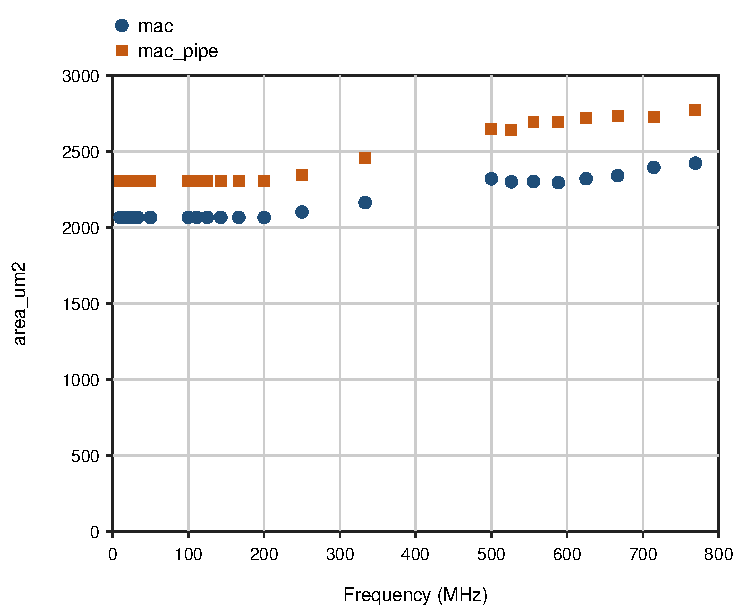
\includegraphics[width=\linewidth]{mac_mac_pipe_freq_MHz_area_um2_MET.pdf}
    }{%
        \caption{Area between \texttt{mac} and \texttt{mac\_pipe} (MET).}
        \label{fig:pipe-area}
    }{%
        \scriptsize
        \begin{tabular}{rrrr}
            \toprule
            \textbf{Freq.\ (MHz)} &
            \multicolumn{2}{c}{\textbf{Area ($\mu m^2$)}} &
            \textbf{$\Delta$Area} \\
            \cmidrule(lr){2-3}
            & \textbf{\texttt{mac}} & \textbf{\texttt{mac\_pipe}} & \\
            \midrule
            10     & 2067.09 & 2306.75 & 239.67 \\
            20     & 2067.09 & 2306.49 & 239.40 \\
            25     & 2067.09 & 2306.49 & 239.40 \\
            50     & 2067.09 & 2306.49 & 239.40 \\
            100    & 2067.09 & 2306.49 & 239.40 \\
            166.67 & 2067.09 & 2306.49 & 239.40 \\
            200    & 2066.29 & 2305.16 & 238.87 \\
            333.33 & 2164.18 & 2459.44 & 295.26 \\
            $\vdots$ & $\vdots$ & $\vdots$ & $\vdots$ \\
            500    & 2320.85 & 2648.03 & 327.18 \\
            526.32 & 2300.90 & 2639.78 & 338.88 \\
            555.56 & 2302.76 & 2692.98 & 390.22 \\
            769.23 & 2424.06 & 2773.58 & 349.52 \\
            \bottomrule
        \end{tabular}
    }{%
        \captionof{table}{Selected MET area points.}
        \label{tab:pipe-area}
    }
\end{figure}

As shown in Figure~\ref{fig:pipe-area}, the area of the pipelined design is generally higher than the unpipelined design, which is expected given the additional pipeline registers. Accounting for increasing in frequency, the area of the pipelined design is about 240 $\mu m^2$ higher than the unpipelined design at 10 MHz, increasing to about 320 $\mu m^2$ at 500 MHz. This trend suggests that the pipelined design is area-deficient at higher frequencies.

An interesting trend in area occurs at the particular frequency from 500MHz to 700MHz. At those frequency the area of the pipelined design increase while the unpipelined design decrease, such that the area difference is significantly greater than at other frequencies. This suggests that pipelined design is more area-deficient at frequencies where the unpipelined design could be optimized to be more area-efficient.

\subsection{Power}

The Total Power is defined the same way as the unpipelined design. Previously, dynamic power was analyzed to cause the trend seen in Figure~\ref{fig:mac-power}. This trend is also seen in Figure~\ref{fig:pipe-power} for the pipelined design.

\begin{figure}[!htbp]
    \plotandtable{%
        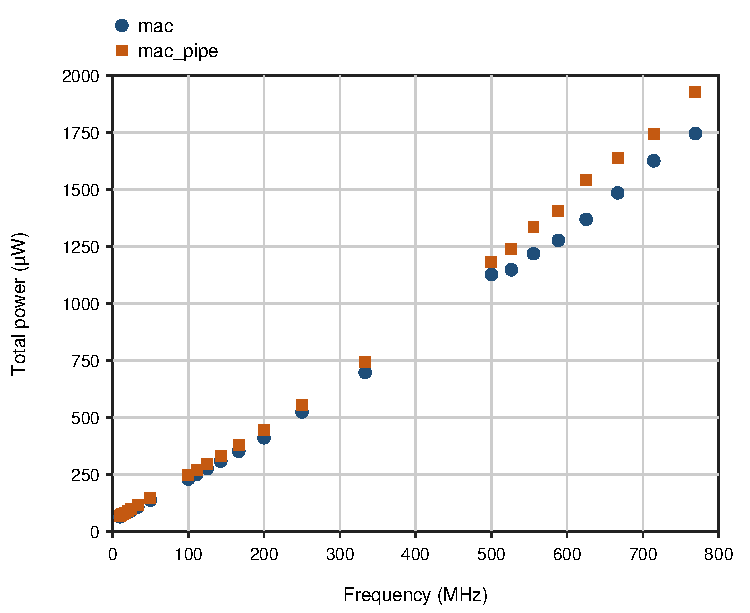
\includegraphics[width=\linewidth]{mac_mac_pipe_freq_MHz_total_uw_MET.pdf}
    }{%
        \caption{Power between \texttt{mac} and \texttt{mac\_pipe} (MET).}
        \label{fig:pipe-power}
    }{%
        \scriptsize
        \begin{tabular}{rrrr}
            \toprule
            \textbf{Freq.\ (MHz)} &
            \multicolumn{2}{c}{\textbf{$\sum$ Power ($\mu W$)}} &
            \textbf{$\Delta$Power} \\
            \cmidrule(lr){2-3}
            & \textbf{\texttt{mac}} & \textbf{\texttt{mac\_pipe}} & \\
            \midrule
            10     & 65.49 & 71.03 & 5.55 \\
            20     & 83.85 & 90.75 & 6.90 \\
            25     & 93.03 & 100.61 & 7.59 \\
            50     & 138.92 & 149.92 & 10.99 \\
            100    & 230.72 & 248.53 & 17.81 \\
            166.67 & 353.12 & 380.01 & 26.89 \\
            200    & 411.86 & 446.49 & 34.63 \\
            333.33 & 698.23 & 744.59 & 46.36 \\
            $\vdots$ & $\vdots$ & $\vdots$ & $\vdots$ \\
            500    & 1127.93 & 1182.18 & 54.26 \\
            526.32 & 1148.45 & 1239.58 & 91.13 \\
            555.56 & 1218.61 & 1333.95 & 115.34 \\
            769.23 & 1745.19 & 1928.30 & 183.11 \\
            \bottomrule
        \end{tabular}
    }{%
        \captionof{table}{Selected MET power points.}
        \label{tab:pipe-power}
    }
\end{figure}

Cell Leakage Power continues to be almost negligible compared with dynamic power, as in the unpipelined design. The slight increase in leakage power for the pipelined design is attributed to the additional pipeline registers increasing the cell area over which leakage can occur. Thus the leakage power could be a more significant fraction in larger designs, especially at lower frequencies. Otherwise, leakage stays approximately constant at low frequency as seen in unpipelined design with the same parameters. The slight increase in power at higher frequency can be attributed to the increased design area from synthesis.

The power difference is minimal at lower frequency, but growing at a larger rate than the unpipelined design. This can be a consequence of the larger pipelined area providing more cells that will be switched each cycle. The rate of power growth becomes more distinct at higher frequency. For example, $\Delta$Power remains on the order of tens of microwatts through 500~MHz and then continues to peak, reaching about 183~$\mu W$ at 769.23~MHz. At this rate, the pipelined design may significantly exceed the power budget compared to the unpipelined design at increasing frequency.

% Make two graphs. On both, show 
% clock frequency on the x­axis; then show area as the y­axis on one graph and power as the y­axis on 
% the other.)

% Explain the trends that you observed and explain why they occur. (

% Only include the design points where the timing constraint is MET

\subsection{Critical Paths}

The start and end points of the critical path for \texttt{mac\_pipe} are reported in Table~\ref{tab:pipe-frequency-area-slack-path}. Because the multiply-add operation is split across two registers, the critical path may lie in either the multiplier stage \texttt{reg1} or the accumulator stage \texttt{reg2}.

\begin{table}[H]
    \centering
    \scriptsize
    \resizebox{\textwidth}{!}{%
    \begin{tabular}{rrrrlll}
        \toprule
        \textbf{Freq.\ (MHz)} &
        \textbf{Area ($\mu m^2$)} &
        \textbf{Power ($\mu W$)} &
        \textbf{Slack (ns)} &
        \textbf{Path Start} &
        \textbf{Path End} &
        \textbf{Timing} \\
        \midrule
        10      & 2306.75 & 71.03   & 95.74  & \texttt{reg2/out\_accum\_reg[0]}  & \texttt{reg2/out\_accum\_reg[47]} & MET \\
        11.11   & 2306.75 & 73.22   & 85.74  & \texttt{reg2/out\_accum\_reg[0]}  & \texttt{reg2/out\_accum\_reg[47]} & MET \\
        12.5    & 2306.49 & 75.96   & 75.74  & \texttt{reg2/out\_accum\_reg[0]}  & \texttt{reg2/out\_accum\_reg[47]} & MET \\
        14.29   & 2306.75 & 79.48   & 65.74  & \texttt{reg2/out\_accum\_reg[0]}  & \texttt{reg2/out\_accum\_reg[47]} & MET \\
        16.67   & 2306.75 & 84.18   & 55.74  & \texttt{reg2/out\_accum\_reg[0]}  & \texttt{reg2/out\_accum\_reg[47]} & MET \\
        20      & 2306.49 & 90.75   & 45.74  & \texttt{reg2/out\_accum\_reg[0]}  & \texttt{reg2/out\_accum\_reg[47]} & MET \\
        25      & 2306.49 & 100.61  & 35.74  & \texttt{reg2/out\_accum\_reg[0]}  & \texttt{reg2/out\_accum\_reg[47]} & MET \\
        33.33   & 2306.49 & 117.05  & 25.74  & \texttt{reg2/out\_accum\_reg[0]}  & \texttt{reg2/out\_accum\_reg[47]} & MET \\
        50      & 2306.49 & 149.92  & 15.74  & \texttt{reg2/out\_accum\_reg[0]}  & \texttt{reg2/out\_accum\_reg[47]} & MET \\
        100     & 2306.49 & 248.53  & 5.74   & \texttt{reg2/out\_accum\_reg[0]}  & \texttt{reg2/out\_accum\_reg[47]} & MET \\
        111.11  & 2306.49 & 270.44  & 4.74   & \texttt{reg2/out\_accum\_reg[0]}  & \texttt{reg2/out\_accum\_reg[47]} & MET \\
        125     & 2306.49 & 297.83  & 3.74   & \texttt{reg2/out\_accum\_reg[0]}  & \texttt{reg2/out\_accum\_reg[47]} & MET \\
        142.86  & 2306.49 & 333.05  & 2.74   & \texttt{reg2/out\_accum\_reg[0]}  & \texttt{reg2/out\_accum\_reg[47]} & MET \\
        166.67  & 2306.49 & 380.01  & 1.74   & \texttt{reg2/out\_accum\_reg[0]}  & \texttt{reg2/out\_accum\_reg[47]} & MET \\
        200     & 2305.16 & 446.49  & 0.75   & \texttt{reg2/out\_accum\_reg[0]}  & \texttt{reg2/out\_accum\_reg[47]} & MET \\
        250     & 2342.93 & 554.37  & 0.12   & \texttt{reg1/out\_product\_reg[0]} & \texttt{reg2/out\_accum\_reg[47]} & MET \\
        333.33  & 2459.44 & 744.59  & 0.00   & \texttt{reg2/out\_accum\_reg[0]}  & \texttt{reg2/out\_accum\_reg[47]} & MET \\
        500     & 2648.03 & 1182.18 & 0.00   & \texttt{reg2/out\_accum\_reg[9]}  & \texttt{reg2/out\_accum\_reg[47]} & MET \\
        526.32  & 2639.78 & 1239.58 & 0.00   & \texttt{reg2/out\_accum\_reg[7]}  & \texttt{reg2/out\_accum\_reg[46]} & MET \\
        555.56  & 2692.98 & 1333.95 & 0.00   & \texttt{input0[7]}  & \texttt{reg1/out\_product\_reg[30]} & MET \\
        588.24  & 2693.52 & 1407.20 & 0.01   & \texttt{input0[3]}  & \texttt{reg1/out\_product\_reg[30]} & MET \\
        625     & 2722.78 & 1541.62 & 0.00   & \texttt{input0[5]}  & \texttt{reg1/out\_product\_reg[30]} & MET \\
        666.67  & 2732.35 & 1636.92 & 0.00   & \texttt{input0[5]}  & \texttt{reg1/out\_product\_reg[29]} & MET \\
        714.29  & 2724.64 & 1741.75 & 0.00   & \texttt{input0[3]}  & \texttt{reg1/out\_product\_reg[30]} & MET \\
        769.23  & 2773.58 & 1928.30 & 0.00   & \texttt{reg2/out\_accum\_reg[7]}  & \texttt{reg2/out\_accum\_reg[47]} & MET \\
        833.33  & 2823.86 & 2116.52 & 0.00   & \texttt{input0[11]} & \texttt{reg1/out\_product\_reg[23]} & VIOLATED\footnotemark \\
        909.09  & 2860.56 & 2372.62 & $-0.06$ & \texttt{input0[13]} & \texttt{reg1/out\_product\_reg[27]} & VIOLATED \\
        1000    & 2832.37 & 2581.64 & $-0.18$ & \texttt{input0[9]}  & \texttt{reg1/out\_product\_reg[20]} & VIOLATED \\
        \bottomrule
    \end{tabular}}
    \caption{Frequency, area, power, timing slack, and critical path for pipelined \texttt{mac\_pipe}.}
    \label{tab:pipe-frequency-area-slack-path} 
\end{table}
\footnotetext{The 833.33~MHz point has a displayed slack of zero but considered as VIOLATED because of negative slack being rounded to zero.}

The additional pipeline register splits the multiply-add operation into two stages, so the critical path may lie in either the multiplier stage or the accumulator stage. At low frequencies and up to around 200~MHz, the critical path is consistently from index~[0] to index~[47] of \texttt{out\_accum\_reg} in \texttt{reg2}. This is likely the path of 48-bit adder carry chain from the least-significant bit of the accumulator to the most-significant bit. At 250~MHz, the cirtical path indictate the carry chain start from the input of the product rather than the accumulator. From 333.33~MHz through 526.32~MHz the path remains in the accumulate stage, with some variation in the start and end indices of \texttt{out\_accum\_reg}. This suggests the carry chain is the main bottleneck at lower frequencies. 

Between 555.56~MHz and 714.29~MHz the critical path moves to the multiplier stage, starting from an \texttt{input0} index and ending at \texttt{reg1/out\_product\_reg}. This indicates the 16$\times$16 multiplier is now the critical path at these frequencies. At 769.23~MHz, the highest frequency that meets timing, the path returns to the accumulate stage. Timing violations from 833.33~MHz onward are again on the multiplier path, from \texttt{input0} to \texttt{reg1/out\_product\_reg}. This suggests the multiplier stage is the bottleneck preventing the design from achieving higher frequency.

%Q3
\section{Performance Comparison}

Both the pipelined and unpipelined design MET the timing constraint at a maximum frequency of 769.23 MHz, corresponding to a period of 1.30 ns. However, the slack violation due to negative rounding indicates that the pipelined design was close to meeting the timing constraint at a period of 1.20 ns. A greater resolution of the clock period may capture a faster pipelined design. 

\begin{table}[H]
    \centering
    \scriptsize
    \resizebox{\textwidth}{!}{%
    \begin{tabular}{lrrrrrlll}
        \toprule
        \textbf{Design} &
        \textbf{Period (ns)} &
        \textbf{Freq.\ (MHz)} &
        \textbf{Area ($\mu m^2$)} &
        \textbf{Power ($\mu W$)} &
        \textbf{Slack (ns)} &
        \textbf{Path Start} &
        \textbf{Path End} &
        \textbf{Timing} \\
        \midrule
        \texttt{mac}       & 1.29 & 775.19 & 2388.68 & 1752.89 & $-0.06$ & \texttt{input0[7]}  & \texttt{acc\_reg[36]} & VIOLATED \\
        \texttt{mac}       & 1.28 & 781.25 & 2401.98 & 1785.59 & $-0.05$ & \texttt{input0[3]}  & \texttt{acc\_reg[26]} & VIOLATED \\
        \texttt{mac}       & 1.27 & 787.40 & 2415.01 & 1802.77 & $-0.04$ & \texttt{input0[6]}  & \texttt{acc\_reg[38]} & VIOLATED \\
        \texttt{mac}       & 1.26 & 793.65 & 2462.89 & 1893.45 & $-0.04$ & \texttt{input0[9]}  & \texttt{acc\_reg[39]} & VIOLATED \\
        \texttt{mac}       & 1.25 & 800.00 & 2445.34 & 1855.99 & $-0.05$ & \texttt{input0[8]}  & \texttt{acc\_reg[43]} & VIOLATED \\
        \texttt{mac}       & 1.24 & 806.45 & 2485.50 & 1892.75 & $-0.05$ & \texttt{input0[5]}  & \texttt{acc\_reg[41]} & VIOLATED \\
        \texttt{mac}       & 1.23 & 813.01 & 2469.28 & 1908.01 & $-0.06$ & \texttt{input0[13]} & \texttt{acc\_reg[42]} & VIOLATED \\
        \texttt{mac}       & 1.22 & 819.67 & 2433.63 & 1872.99 & $-0.07$ & \texttt{input0[1]}  & \texttt{acc\_reg[42]} & VIOLATED \\
        \texttt{mac}       & 1.21 & 826.45 & 2441.61 & 1933.98 & $-0.04$ & \texttt{input0[6]}  & \texttt{acc\_reg[23]} & VIOLATED \\
        \midrule
        \texttt{mac\_pipe} & 1.21 & 826.45 & 2810.29 & 2122.06 & 0.00    & \texttt{input0[8]}  & \texttt{reg1/out\_product\_reg[25]} & MET \\
        \bottomrule
    \end{tabular}}
    \caption{Fine-period area, power, slack, and timing for maximum frequency.}
    \label{tab:max-freq}
\end{table}

As shown in Table~\ref{tab:max-freq}, the pipelined design is able to meet a stricter timing constraint with a clock period of 1.21~ns. Where the unpipelined design is VIOLATED at 1.21~ns, the pipelined design MET the timing constraints to run at a faster frequency of 826.45~MHz. Therefore the additional pipeline register provide a modest 60MHz improvement in frequency compared to the unpipelined design. The critical path is still from \texttt{input0} to \texttt{reg1/out\_product\_reg} at 826.45~MHz, indicating the multiplier stage is still the bottleneck of the pipelined design. Achievement in higher frequency may be possible with deeper pipelining of the multiplier stage.

For now, we will use the pipelined design at a clock period of 1.21~ns or 826.45~MHz as the maximum clock frequency for the following analysis.

%Q4
\subsection{Maximum-Frequency Energy}

Energy is the integral of power over time. Synthesis reports average power,
\[
P_\mathrm{avg} = \frac{1}{T}\int_0^{T} P(t)\,dt,
\]
in Watts as Joules per second. Using the maximum frequency case from Table~\ref{tab:max-freq}, $P_\mathrm{avg}$ is the total power of the \texttt{mac\_pipe} design. The time is the clock period used that MET the timing constraint for \texttt{mac\_pipe}, where the clock period is $t = 1.21$~ns for the maximum frequency case. Therefore, the energy of a single clock cycle is 

\[
E_\mathrm{cycle} = P_\mathrm{avg}\,t.
\]


Suppose we want to compute 50 sets of input values. The 2-stage \texttt{mac\_pipe} design will take one additional cycle to fill the pipeline with inputs before the outputs could be computed every cycle. Then the total time to compute 50 sets will require 51 cycles. Thus, the energy consumed for 50 sets of input is

\begin{align*}
E = 51 (E_\mathrm{cycle}) &= 51 (P_\mathrm{avg}\,t) \\
&= 51 (2.122 \times 10^{-3}~\mathrm{W} \times 1.21 \times 10^{-9}~\mathrm{s}) \\
&= 1.31 \times 10^{-10}~\mathrm{J}.
\end{align*}

This is equivalent to about 131 pico-Joules of energy consumed to compute 50 sets of input values.



%Q5
\subsection{Frequency-Dependent Energy}
% Would  the  energy  you  computed  in  question  3  change  if  you  resynthesized  the  design  targeting different clock frequencies? Explain and justify your answer. 

%Think carefully about what changes when you change the target frequency and how those changes affect the power the system consumes.

\subsection{Latency and Throughput}
% Make a table that compares the power, area, latency, and throughput of your pipelined and unpipelined 
% MAC designs

% In your report show how you calculated the latency and throughput. Quantify latency in seconds  (or  ns),  and  quantify  throughput  in  terms  of  MACs  per  second. TOPIC 6

\subsection{Design Trade-offs}

% Based  on  the  trade­offs  seen  in  your  table,  explain  when  it  would 
% make sense for a designer to choose the pipelined design and when it would make sense to use the 
% unpipelined design

%Q6
\section{Potential for Deeper Pipelining}

\subsection{Multiplier Pipelining}

% Based on your 
% results to questions 1 and 2, would you expect that deeper pipelining in the multiplier might help you 
% reach higher clock frequencies? Justify why or why not.

% If you were to pipeline the multiplier in this way, what other changes would you have to make in your 
% module? Be specific about each of the module’s control inputs: which of them would need to change, 
% and which would not?

\subsection{Adder Pipelining}
% Would pipelining inside of the adder be possible and a good idea? Why or why not?

% Answer this question based on your understanding of the design and your answers to prior questions. 
% You do not need to modify your design/code to answer this question.

%Q7
\section{Variable Parameter Synthesis Results}

% how changing WIDTH and ACCW affects the critical path location and maximum clock frequency of your pipelined MAC module

%Q7
\subsection{Accumulator Width (ACCW)}
% First, do a set of experiments where you set WIDTH=12 and synthesize three designs with ACCW=24, 48, 
% and 64

%Q7
\subsection{Numerical-Bit Width (WIDTH)}
% Next, do a new set of experiments where you set ACCW=48 and synthesize three designs with WIDTH=8, 
% 16, 24.

\subsection{Scaling Behavior}
% Do  the  clock  frequency  and  critical  path  location  change  as  ACCW  changes? 

% Do  the  clock  frequency  and  critical  path location change  when 
% WIDTH changes?

% Explain what you see and what you learn from it. You should expect to see differences in the scaling behavior of WIDTH and ACCW. 

% Explain why they behave differently. In your explanation, account for the shift­and­saturate logic on the output path as well as the multiplier and adder.

%Q8
\subsection{Accumulator Overflow}

%if the value stored in the accumulator grows large enough, it will overflow. That is, ACCW bits may not be enough to store the resulting number.

% Assume WIDTH=5 and ACCW=16. What is the maximum number of MACs your system could perform while guaranteeing that the accumulator cannot overflow?

% what is the largest magnitude number you could produce on the multiplier’s output? Then, how many accumulations would it take for that number to produce an overflow in the accumulator? 

% Don’t forget that our values are all signed integers, and  don’t  forget  that  the  accumulator  can  be  initialized  to  a  signed  WIDTH­bit  number.  Show  your reasoning and justify your answer.

\section{Appendix}
% Include the six synthesis reports for parameter scaling along with the report.

\end{document}
